% Options for packages loaded elsewhere
\PassOptionsToPackage{unicode}{hyperref}
\PassOptionsToPackage{hyphens}{url}
\PassOptionsToPackage{dvipsnames,svgnames,x11names}{xcolor}
%
\documentclass[
  letterpaper,
  DIV=11,
  numbers=noendperiod]{scrartcl}

\usepackage{amsmath,amssymb}
\usepackage{iftex}
\ifPDFTeX
  \usepackage[T1]{fontenc}
  \usepackage[utf8]{inputenc}
  \usepackage{textcomp} % provide euro and other symbols
\else % if luatex or xetex
  \usepackage{unicode-math}
  \defaultfontfeatures{Scale=MatchLowercase}
  \defaultfontfeatures[\rmfamily]{Ligatures=TeX,Scale=1}
\fi
\usepackage{lmodern}
\ifPDFTeX\else  
    % xetex/luatex font selection
\fi
% Use upquote if available, for straight quotes in verbatim environments
\IfFileExists{upquote.sty}{\usepackage{upquote}}{}
\IfFileExists{microtype.sty}{% use microtype if available
  \usepackage[]{microtype}
  \UseMicrotypeSet[protrusion]{basicmath} % disable protrusion for tt fonts
}{}
\makeatletter
\@ifundefined{KOMAClassName}{% if non-KOMA class
  \IfFileExists{parskip.sty}{%
    \usepackage{parskip}
  }{% else
    \setlength{\parindent}{0pt}
    \setlength{\parskip}{6pt plus 2pt minus 1pt}}
}{% if KOMA class
  \KOMAoptions{parskip=half}}
\makeatother
\usepackage{xcolor}
\setlength{\emergencystretch}{3em} % prevent overfull lines
\setcounter{secnumdepth}{5}
% Make \paragraph and \subparagraph free-standing
\ifx\paragraph\undefined\else
  \let\oldparagraph\paragraph
  \renewcommand{\paragraph}[1]{\oldparagraph{#1}\mbox{}}
\fi
\ifx\subparagraph\undefined\else
  \let\oldsubparagraph\subparagraph
  \renewcommand{\subparagraph}[1]{\oldsubparagraph{#1}\mbox{}}
\fi


\providecommand{\tightlist}{%
  \setlength{\itemsep}{0pt}\setlength{\parskip}{0pt}}\usepackage{longtable,booktabs,array}
\usepackage{calc} % for calculating minipage widths
% Correct order of tables after \paragraph or \subparagraph
\usepackage{etoolbox}
\makeatletter
\patchcmd\longtable{\par}{\if@noskipsec\mbox{}\fi\par}{}{}
\makeatother
% Allow footnotes in longtable head/foot
\IfFileExists{footnotehyper.sty}{\usepackage{footnotehyper}}{\usepackage{footnote}}
\makesavenoteenv{longtable}
\usepackage{graphicx}
\makeatletter
\def\maxwidth{\ifdim\Gin@nat@width>\linewidth\linewidth\else\Gin@nat@width\fi}
\def\maxheight{\ifdim\Gin@nat@height>\textheight\textheight\else\Gin@nat@height\fi}
\makeatother
% Scale images if necessary, so that they will not overflow the page
% margins by default, and it is still possible to overwrite the defaults
% using explicit options in \includegraphics[width, height, ...]{}
\setkeys{Gin}{width=\maxwidth,height=\maxheight,keepaspectratio}
% Set default figure placement to htbp
\makeatletter
\def\fps@figure{htbp}
\makeatother

\usepackage{lineno,setspace}
\linenumbers
\doublespacing
\KOMAoption{captions}{tableheading}
\renewcommand{\figurename}{Figure}
\renewcommand{\thefigure}{S\arabic{figure}}
\makeatletter
\@ifpackageloaded{caption}{}{\usepackage{caption}}
\AtBeginDocument{%
\ifdefined\contentsname
  \renewcommand*\contentsname{Table of contents}
\else
  \newcommand\contentsname{Table of contents}
\fi
\ifdefined\listfigurename
  \renewcommand*\listfigurename{List of Figures}
\else
  \newcommand\listfigurename{List of Figures}
\fi
\ifdefined\listtablename
  \renewcommand*\listtablename{List of Tables}
\else
  \newcommand\listtablename{List of Tables}
\fi
\ifdefined\figurename
  \renewcommand*\figurename{Figure}
\else
  \newcommand\figurename{Figure}
\fi
\ifdefined\tablename
  \renewcommand*\tablename{Table}
\else
  \newcommand\tablename{Table}
\fi
}
\@ifpackageloaded{float}{}{\usepackage{float}}
\floatstyle{ruled}
\@ifundefined{c@chapter}{\newfloat{codelisting}{h}{lop}}{\newfloat{codelisting}{h}{lop}[chapter]}
\floatname{codelisting}{Listing}
\newcommand*\listoflistings{\listof{codelisting}{List of Listings}}
\makeatother
\makeatletter
\makeatother
\makeatletter
\@ifpackageloaded{caption}{}{\usepackage{caption}}
\@ifpackageloaded{subcaption}{}{\usepackage{subcaption}}
\makeatother
\ifLuaTeX
  \usepackage{selnolig}  % disable illegal ligatures
\fi
\usepackage{bookmark}

\IfFileExists{xurl.sty}{\usepackage{xurl}}{} % add URL line breaks if available
\urlstyle{same} % disable monospaced font for URLs
\hypersetup{
  pdftitle={Supplemental information for neonSoilFlux: An R Package for Continuous Sensor-Based Estimation of Soil CO2 Fluxes},
  pdfauthor={, , , , , , , , , , , and },
  colorlinks=true,
  linkcolor={blue},
  filecolor={Maroon},
  citecolor={Blue},
  urlcolor={Blue},
  pdfcreator={LaTeX via pandoc}}

\title{Supplemental information for \texttt{neonSoilFlux}: An R Package
for Continuous Sensor-Based Estimation of Soil CO\textsubscript{2}
Fluxes}
\author{John Zobitz\textsuperscript{1} \and Ed
Ayres\textsuperscript{2} \and Zoey Werbin\textsuperscript{3} \and Ridwan
Abdi\textsuperscript{1} \and Natalie
Ashburner-Wright\textsuperscript{4} \and Lillian
Brown\textsuperscript{4} \and Ryan
Frink-Sobierajski\textsuperscript{4} \and Lajntxiag
Lee\textsuperscript{1} \and Dijonë
Mehmeti\textsuperscript{1} \and Christina
Tran\textsuperscript{4} \and Ly Xiong\textsuperscript{1} \and Naupaka
Zimmerman\textsuperscript{4,5}}
\date{}

\begin{document}
\maketitle

\textsuperscript{1} Augsburg University, 2211 Riverside Avenue,
Minneapolis, MN 55454\\
\textsuperscript{2} National Ecological Observatory Network, Battelle,
1685 38th Street, Suite 100, Boulder, CO 80301\\
\textsuperscript{3} Boston University, 5 Cummington Street, Boston, MA
02215\\
\textsuperscript{4} University of San Francisco, 2130 Fulton Street, San
Francisco, CA 94117\\
\textsuperscript{5} University of Kansas, 1251 Wescoe Dr.~Lawrence, KS
66045

\section{Assessment of data gaps}\label{assessment-of-data-gaps}

For a given half-hourly time period, the \texttt{neonSoilFlux} packages
assigns a QA flag for a measurement if more one values across all
measurement depths uses gap-filled data (Section 4.2.1 of the main
text). Panel a of Figure~\ref{fig-gap-filled-stats} reports the
proportion of gap-filled data for all input environmental measurements
at each site during the period when field measurements were made. Soil
fluxes are computed from 4 different types of input measurements
(\(T_{S}\), \(SWC\), \(P\), and CO\(_{2}\)), any of which could have a
QA flag in a half-hourly interval. Panel b of
Figure~\ref{fig-gap-filled-stats} displays at each site the distribution
of the number of different gap-filled measurements used to compute a
half-hourly flux. The largest cause of measurements needing to be
gap-filled was missing or flagged soil moisture data. Calculating fluxes
for WOOD and SJER required using the largest proportion of gap-filled
measurements, due to substantially large fractions of flagged or missing
\(SWC\) and \(T_{S}\) data.

\begin{figure}

\centering{

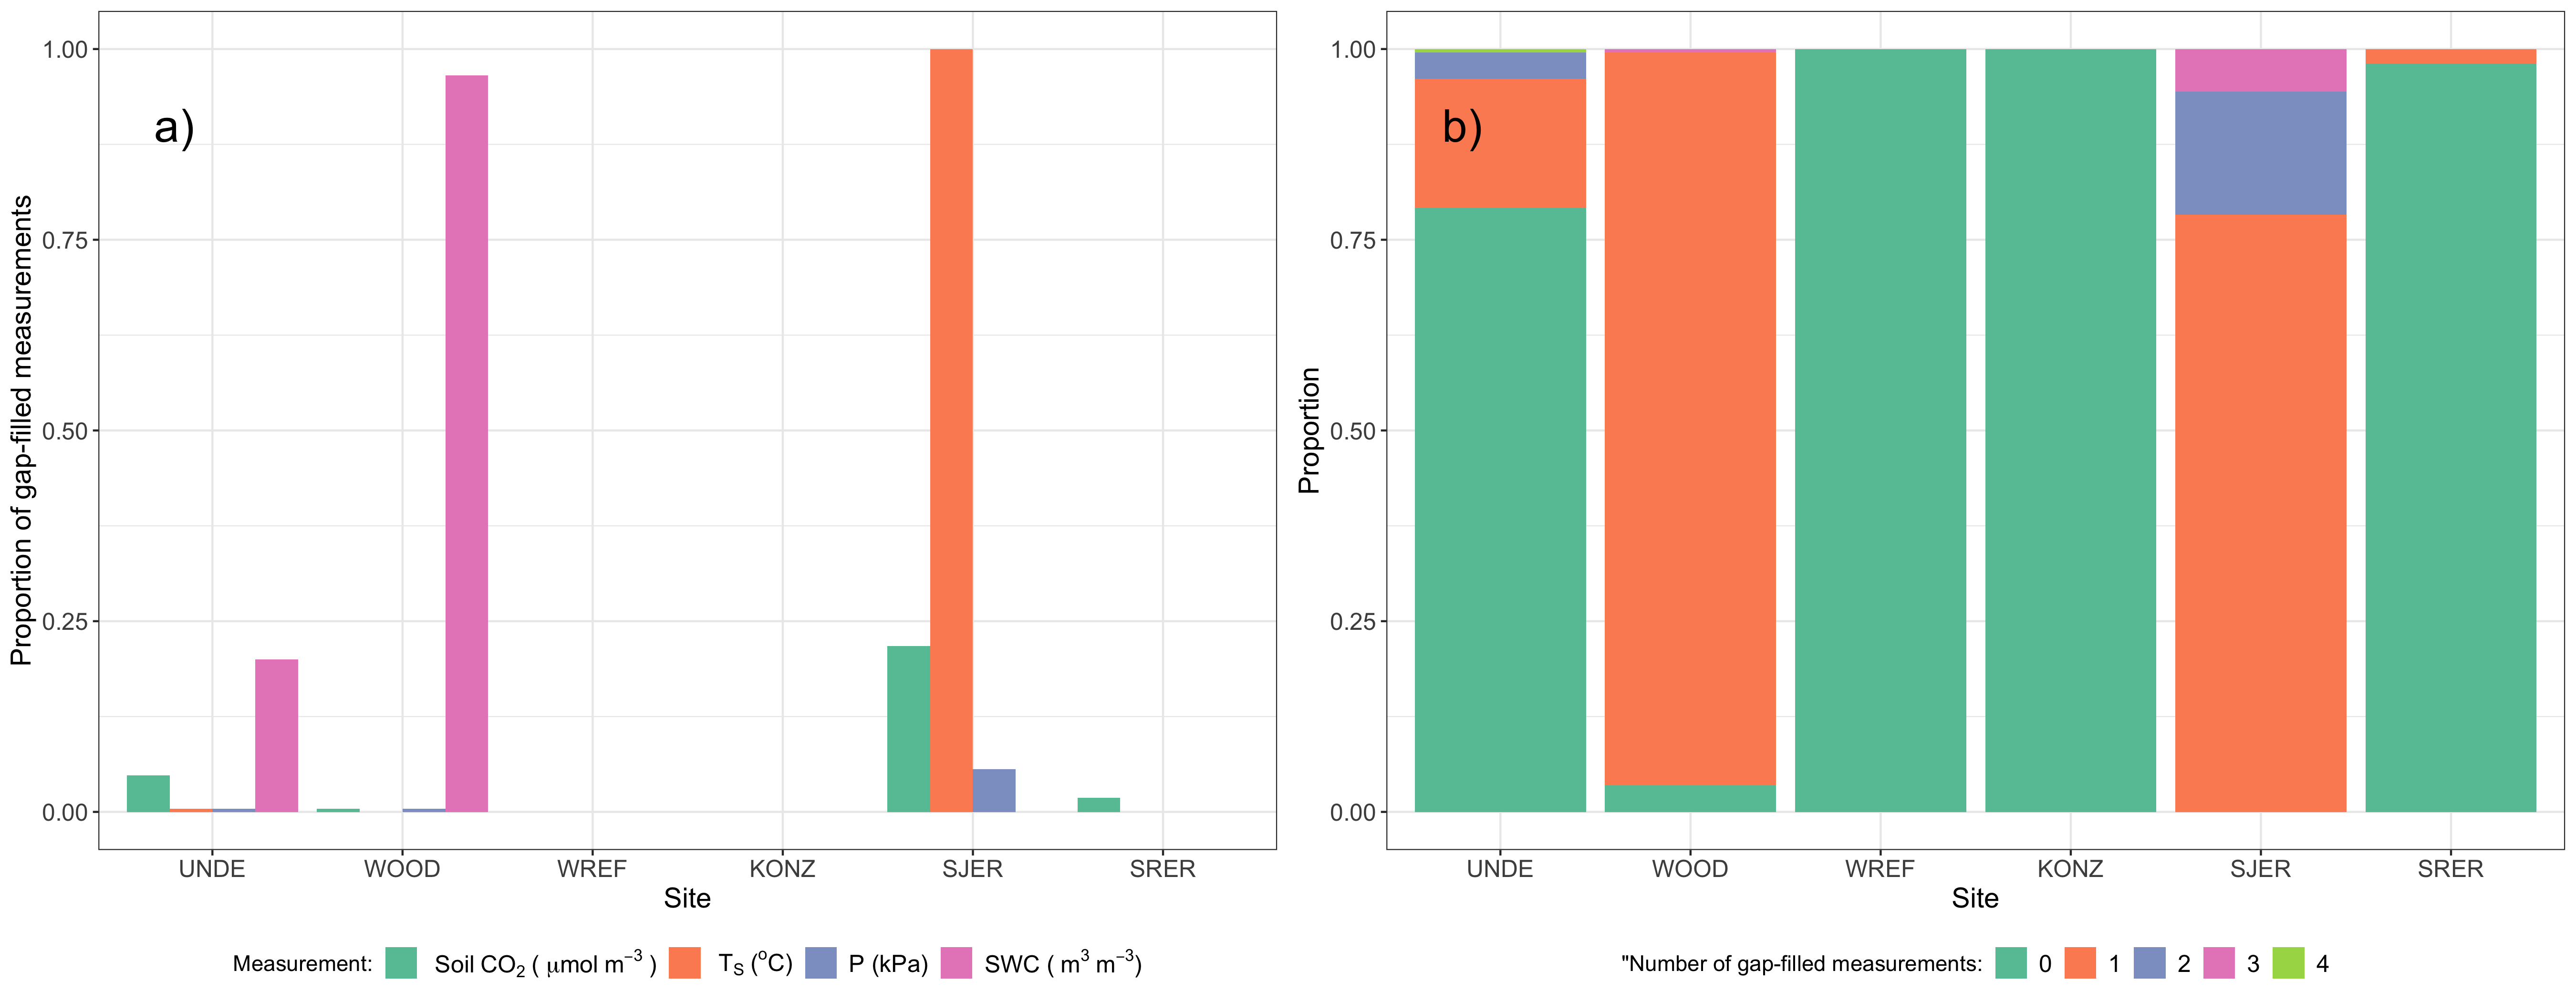
\includegraphics{figures/gap-filled-stats.png}

}

\caption{\label{fig-gap-filled-stats}Panel a) Proportion of input
gap-filled environmental measurements used to generate \(F_{S}\) from
the \texttt{neonSoilFlux} package, by study site. Panel b) distribution
of the usage of gap-filled measurements at each site.}

\end{figure}%

\section{Assessing the signal to noise ratio (SNR) and evaluating
estimated
uncertainties}\label{assessing-the-signal-to-noise-ratio-snr-and-evaluating-estimated-uncertainties}

Following collection of field measurements and calculation of the soil
fluxes from \texttt{neonSoilFlux} package, we compared measured
\(F_{S}\) based on closed-dynamic chamber measurements with the LI-COR
instruments to a given soil flux calculation from \texttt{neonSoilFlux}
for each site and flux computation method. Beyond the model statistics
defined in the main text, we computed the signal to noise ratio (SNR),
defined as the ratio of a modeled soil flux (\(F_{ijk}\)) from
\texttt{neonSoilFlux} to its quadrature uncertainty (\(\sigma_{ijk}\)).

We observed that the range of values (e.g.~\(F_{ijk} \pm \sigma_{ijk}\)
was much larger than the measured field flux. We evaluated
\(| F_{S} - F_{ijk} | < (1-\epsilon) \sigma_{ijk}\), where \(F_{S}\) is
a measured field soil flux from the LI-COR 6800 (as the LI-COR 870/8250
was used at only three sites in 2024 but the 6800 was used at all sites
in both years). The parameter \(\epsilon\) was an uncertainty reduction
factor to evaluate how much the quadrature uncertainty could be reduced
while maintaining precision between modeled \(F_{ijk}\) and measured
\(F_{S}\).

The computed signal to noise ratio (SNR) and the proportion of measured
field fluxes within the modeled uncertainty for a given flux computation
method \(F_{ijk}\) suggest that there was substantial variability in the
agreement between the gradient method and field-measured observations
(Figure~\ref{fig-uncertainty-stats}, Section 4.3 of the main text).
Here, values of SNR greater than unity indicate lower reported
uncertainty, as propagated by quadrature due to a relatively higher
precision of measured input variables (CO\(_{2}\), \(T_{S}\), \(SWC\),
or \(P\)).

The sensitivity to an uncertainty reduction factor (\(\epsilon\), bottom
panels in Figure~\ref{fig-uncertainty-stats}) demonstrates how
concordance between measured and modeled fluxes would be affected if
environmental measurement uncertainty \(\sigma_{ijk}\) were to decrease.
As \(\epsilon\) increases from left to right in each figure, the
possible range of values for each predicted flux value decreases and the
proportion of measured fluxes that fall within that range also
decreases.

\begin{figure}

\centering{

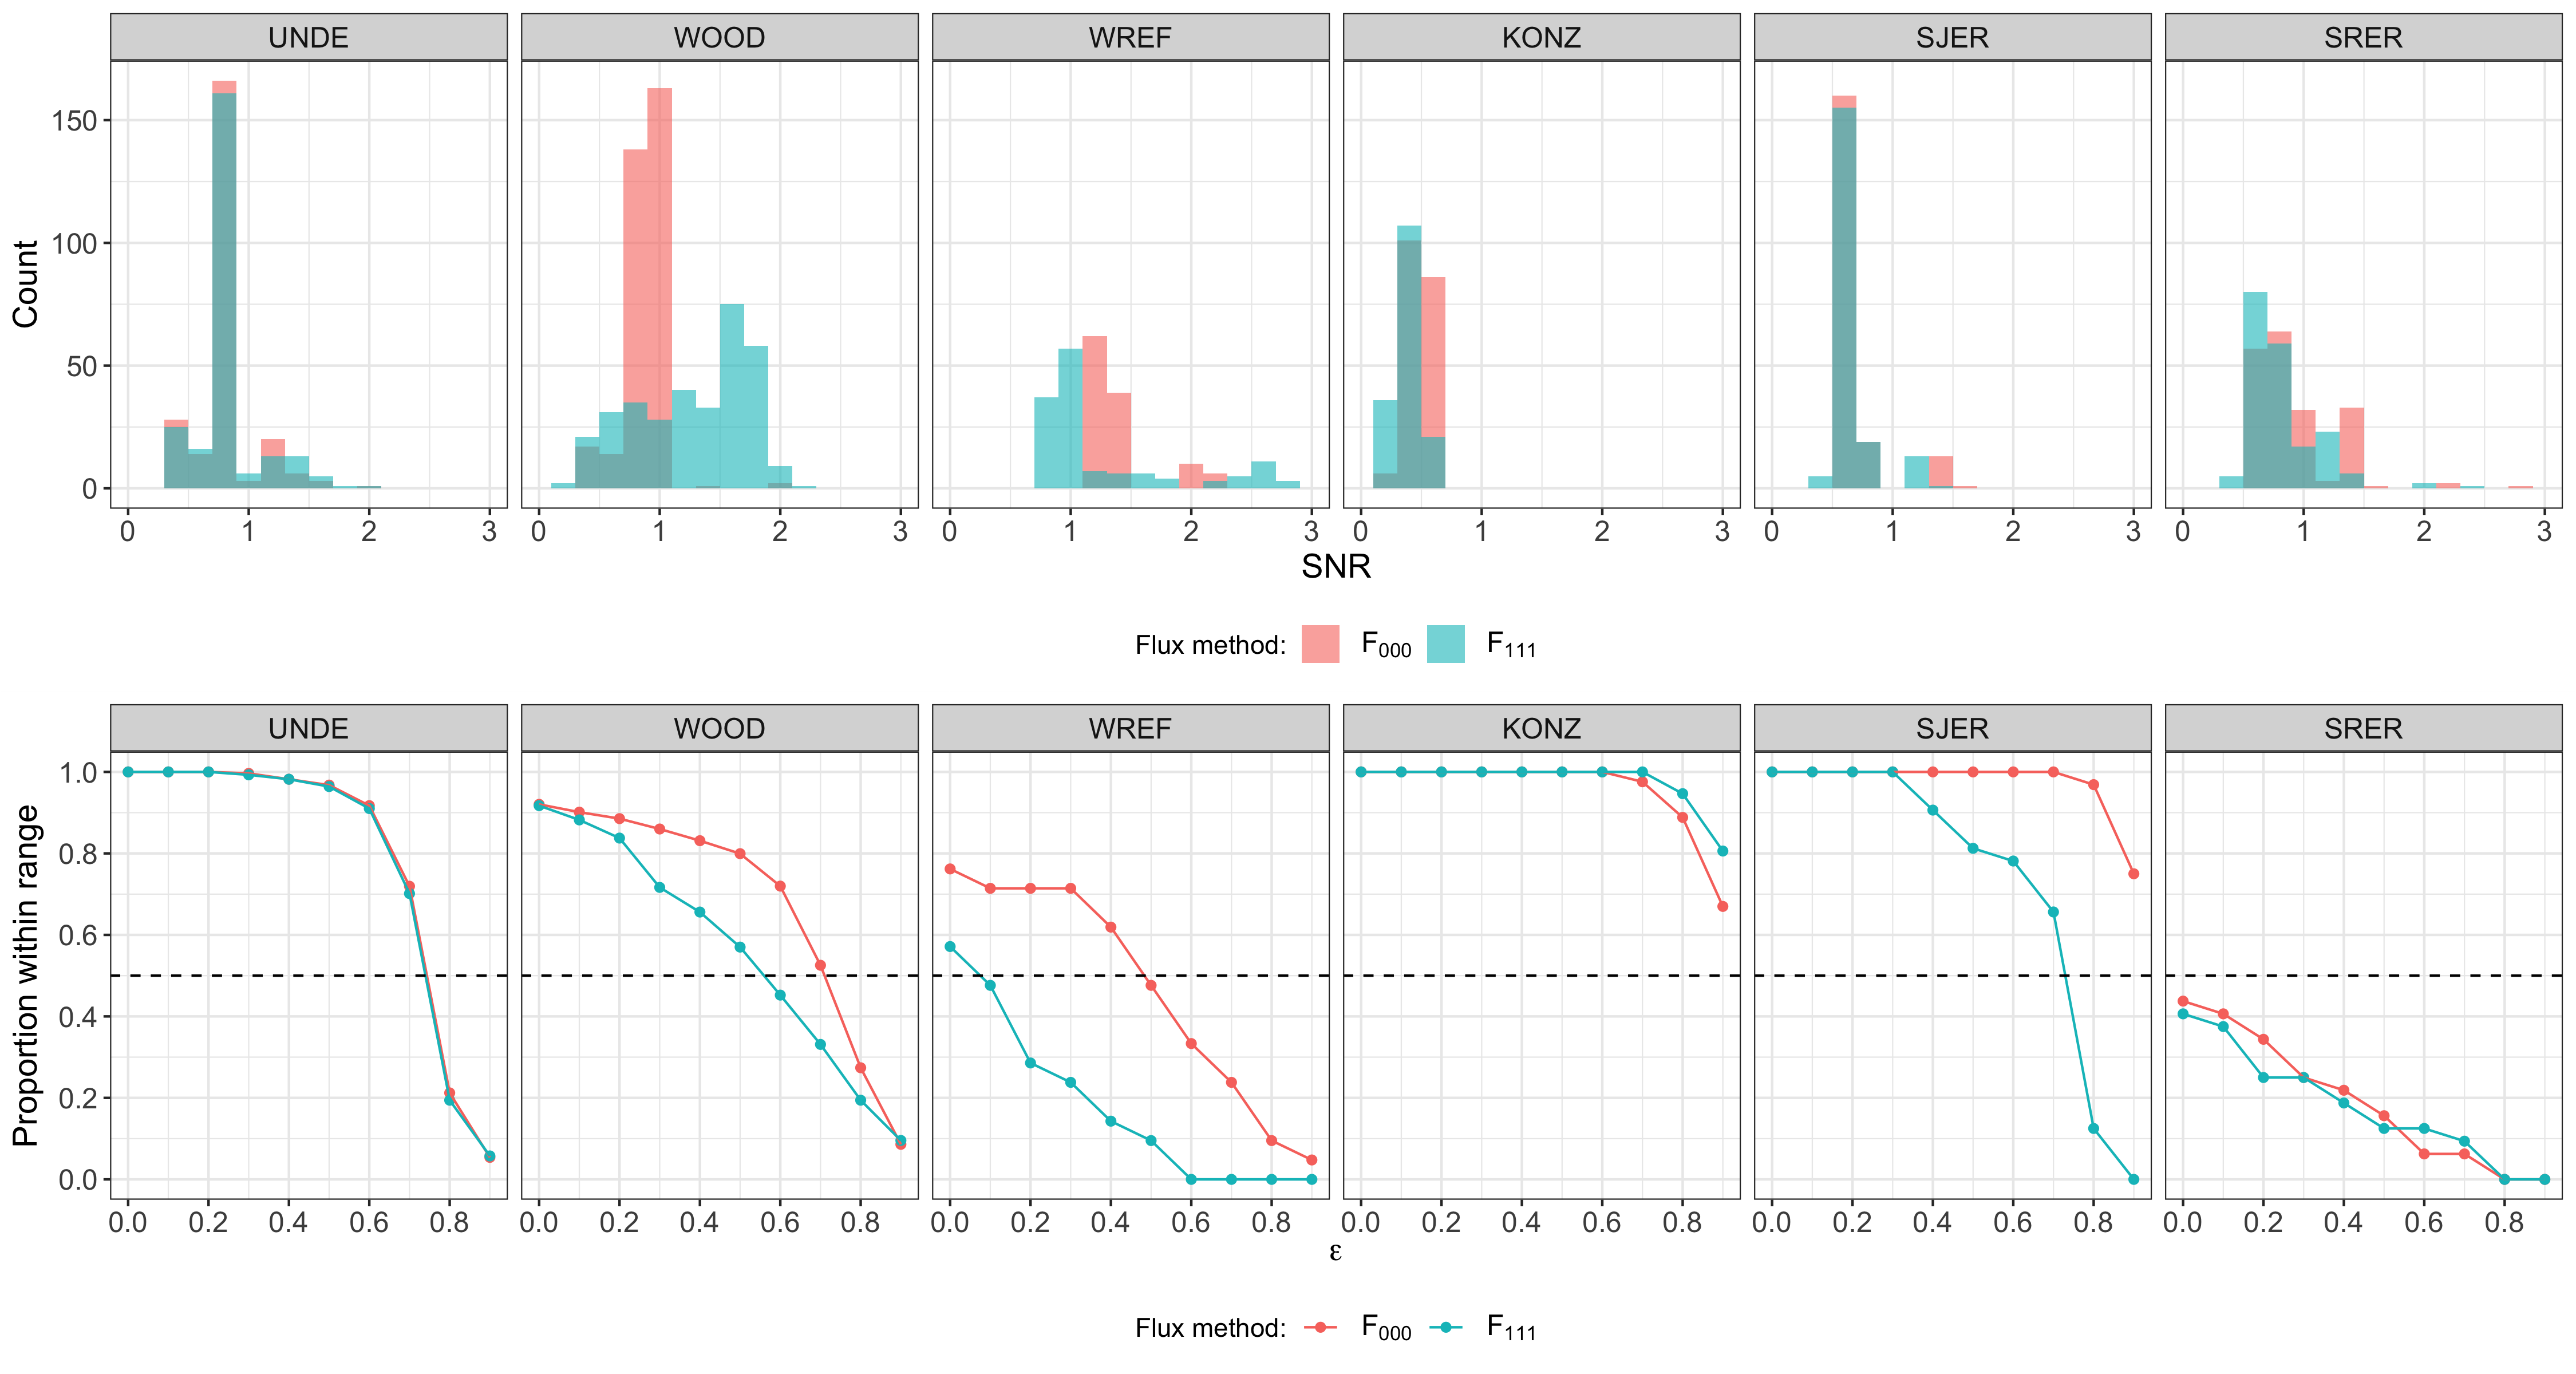
\includegraphics{figures/uncertainty-stats.png}

}

\caption{\label{fig-uncertainty-stats}Top panels: distribution of SNR
values across each of the different sites for modeled effluxes from the
\texttt{neonSoilFlux} package, depending on the diffusivity calculation
used (Millington-Quirk or Marshall, Section 4.2.2 of the main text).
Bottom panels: Proportion of measured \(F_{S}\) within the modeled range
of a flux computation method \(F_{ijk}\) given an uncertainty reduction
factor \(\epsilon\), or
\(| F_{S} - F_{ijk} | < (1-\epsilon) \sigma_{ijk}\).}

\end{figure}%



\end{document}
